\documentclass{article}
\usepackage[a4paper, landscape]{geometry}
\usepackage{multicol}
\usepackage{amsmath,amssymb}
\usepackage{tikz}
\usetikzlibrary{decorations.pathmorphing,shapes.geometric}
\usepackage{xcolor}
\usepackage{enumitem}
\usepackage{colortbl}
\usepackage{array}
\usepackage{hyperref}
\usepackage{fontspec}

\setmainfont{Atkinson Hyperlegible}

% Page layout adjustments
\setlength{\topmargin}{-30mm}
\setlength{\textheight}{200mm}
\setlength{\textwidth}{287mm}
\setlength{\oddsidemargin}{-25mm}
\setlength{\evensidemargin}{-25mm}

% TikZ styles
\tikzstyle{mybox} = [draw=black, fill=white, very thick, rectangle, rounded corners, inner sep=10pt, inner ysep=10pt]
\tikzstyle{fancytitle} =[fill=black, text=white, font=\bfseries]

\begin{document}

\begin{center}{\huge{\textbf{Cooking Cheatsheet}}}\end{center}
\vspace{1mm}
\raggedcolumns
\begin{multicols*}{3}

\begin{tikzpicture}
\node [mybox] (box){%
    \begin{minipage}{0.3\textwidth}
        \textbf{Volume Conversions:}
        
        \begin{tabular}{|c|c|}
        \hline
        1 Cup & 240 ml \\
        1 Tablespoon & 15 ml \\
        1 Teaspoon & 5 ml \\
        1 Cup & 16 Tablespoons \\
        1 Tablespoon & 3 Teaspoons \\
        1 Liter & 4.2 Cups \\
        \hline
        \end{tabular}
        
        \textbf{Weight Conversions:}
        
        \begin{tabular}{|c|c|}
        \hline
        1 lb (pound) & 453.6 g \\
        1 kg & 2.2 lbs \\
        1 oz (ounce) & 28.3 g \\
        \hline
        \end{tabular}
    \end{minipage}
};
\node[fancytitle, right=10pt] at (box.north west) {Measurement Conversions};
\end{tikzpicture}

% Temperature Conversions
\begin{tikzpicture}
\node [mybox] (box){%
    \begin{minipage}{0.3\textwidth}
        \[ C = \frac{(F-32) \times 5}{9} \]
        
        \textbf{Oven Temperatures:}
        
        \begin{tabular}{|c|c|c|}
        \hline
        \textbf{Description} & \textbf{°F} & \textbf{°C} \\
        \hline
        Low & 250-300 & 120-150 \\
        Moderate & 350-375 & 175-190 \\
        Hot & 400-425 & 200-220 \\
        Very Hot & 450-475 & 230-245 \\
        \hline
        \end{tabular}
    \end{minipage}
};
\node[fancytitle, right=10pt] at (box.north west) {Temperature Guide};
\end{tikzpicture}

\begin{tikzpicture}
\node [mybox] (box){%
    \begin{minipage}{0.3\textwidth}
        \textbf{Safe Internal Meat Temperatures:}
        
        \begin{tabular}{|l|c|}
        \hline
        \textbf{Meat} & \textbf{Safe Temp (°C)} \\
        \hline
        Chicken & 74 \\
        Turkey & 74 \\
        Ground Beef & 71 \\
        Beef Steaks/Roasts & 63 \\
        Pork & 63 \\
        Fish & 63 \\
        \hline
        \end{tabular}
        
        \textbf{Beef Doneness Temperatures:}
        
        \begin{tabular}{|l|c|}
        \hline
        \textbf{Doneness} & \textbf{Temp (°C)} \\
        \hline
        Rare & 52-55 \\
        Medium Rare & 55-60 \\
        Medium & 60-65 \\
        Medium Well & 65-70 \\
        Well Done & 70-75 \\
        \hline
        \end{tabular}
    \end{minipage}
};
\node[fancytitle, right=10pt] at (box.north west) {Cooking Temperatures};
\end{tikzpicture}

% Spice Pairings
\begin{tikzpicture}
\node [mybox] (box){%
    \begin{minipage}{0.3\textwidth}
        \textbf{Spice Pairings:}
        
        \begin{tabular}{|l|l|}
        \hline
        \textbf{Protein} & \textbf{Spices} \\
        \hline
        Chicken & Thyme, Rosemary \\
        Beef & Rosemary, Garlic \\
        Fish & Dill, Lemon Pepper \\
        Pork & Sage, Fennel \\
        \hline
        \end{tabular}
        
        \textbf{Cultural Flavor Guide:}
        
        \begin{tabular}{|l|l|}
        \hline
        \textbf{Cuisine} & \textbf{Key Spices/Herbs} \\
        \hline
        Mexican & Cumin, Chili, Oregano \\
        Italian & Basil, Oregano, Thyme \\
        Indian & Turmeric, Cumin, Coriander \\
        Thai & Lemongrass, Ginger, Chili \\
        Mediterranean & Za'atar, Mint, Sumac \\
        \hline
        \end{tabular}
    \end{minipage}
};
\node[fancytitle, right=10pt] at (box.north west) {Spice Guide};
\end{tikzpicture}

\begin{tikzpicture}
\node [mybox] (box){%
    \begin{minipage}{0.3\textwidth}
        \begin{tabular}{|l|l|}
        \hline
        \textbf{Ingredient} & \textbf{Substitute} \\
        \hline
        1 Egg & 60 ml applesauce \\
        Buttermilk & Milk + Vinegar \\
        Butter & Applesauce, Oils \\
        Flour & Almond meal \\
        \hline
        \end{tabular}
    \end{minipage}
};
\node[fancytitle, right=10pt] at (box.north west) {Baking Substitutes};
\end{tikzpicture}

\begin{tikzpicture}
\node [mybox] (box){%
    \begin{minipage}{0.3\textwidth}
        \textbf{Common Ratios:}
        
        \begin{tabular}{|l|c|}
        \hline
        \textbf{Recipe} & \textbf{Ratio} \\
        \hline
        Vinaigrette & 3:1 (Oil:Vinegar) \\
        Marinade & 3:1:1 (Oil:Acid:Seasoning) \\
        Stock/Broth & 1.8 kg bones: 3.8 L water \\
        \hline
        \end{tabular}
        
        \textbf{Grain Cooking Ratios:}
        
        \begin{tabular}{|l|c|c|}
        \hline
        \textbf{Grain} & \textbf{Water Ratio} & \textbf{Time} \\
        \hline
        Rice (White) & 2:1 & 18-20 min \\
        Rice (Brown) & 2.5:1 & 45-50 min \\
        Quinoa & 2:1 & 15-20 min \\
        Pasta & N/A & 8-12 min \\
        \hline
        \end{tabular}
    \end{minipage}
};
\node[fancytitle, right=10pt] at (box.north west) {Cooking Ratios};
\end{tikzpicture}

\begin{tikzpicture}
\node [mybox] (box){%
    \begin{minipage}{0.3\textwidth}
        \begin{itemize}[leftmargin=*]
            \item Oversalted: Add acid/fat
            \item Bland: Add herbs, salt
            \item Burnt: Scrape off, add sauce
        \end{itemize}
    \end{minipage}
};
\node[fancytitle, right=10pt] at (box.north west) {Cooking Fixes};
\end{tikzpicture}

\begin{tikzpicture}
\node [mybox] (box){%
    \begin{minipage}{0.3\textwidth}
        \begin{tabular}{|l|c|c|}
        \hline
        \textbf{Item} & \textbf{Fridge} & \textbf{Freezer} \\
        \hline
        Raw Chicken & 1-2 days & 9 months \\
        Cooked Meat & 3-4 days & 2-6 months \\
        Fresh Eggs & 3-5 weeks & Not Recommended \\
        Milk & 7 days & 3 months \\
        \hline
        \end{tabular}
    \end{minipage}
};
\node[fancytitle, right=10pt] at (box.north west) {Food Storage};
\end{tikzpicture}

\end{multicols*}
\end{document}
